\chapter{Neutrino as Astroparticle}
\label{chap:neutrino}
When looking at phenomena outside our earth the astronomer will turn to
electromagnetic radiation, but he's missing out on a big part of the full
picture. Not only do interesting events emit photons but also muons, nuclei,
gravitational waves,... All kinds of particles which might also be of interest,
that's where the astroparticle physicist comes in.

Of all these particles there is one particle which has properties we're quite
interested in: the neutrino.  Neutrinos don't have any charge, meaning that
they are not deflected by magnetic fields. Also neutrinos interact very weakly,
because of this they are often called “ghost” particles; on average 100
trillion neutrinos pass through your body per second, none of them having any
effect.  You'd even need a light year of lead to give you just a 50\% chance of
stopping a neutrino.
These properties make them ideal messenger particles as, when we detect a neutrino
and its arrival direction, we can be quite sure it came to our detector unhindered
from a far away event in the exact same direction.
Neutrinos can serve as unique clues
about what’s happening elsewhere in the universe including the cosmic
collisions, galaxies, supernovae, Gamma-ray bursts (GRBs),... Where they are created.

In this chapter we'll give an overview of neutrinos and the various kinds of energies we expect
to see them in when coming from outside our earth.

\section{Discovery}
In the fifties researchers were investigating $\beta^-$ decay, the decay of a neutron. 
In the proton-electron model for the $\beta^-$-decay of a nucleus (A,Z) you would
expect the final result to be (A,Z+1) + $e^-$, or
\begin{equation}
	n \rightarrow p^+ + e^-
\end{equation}
However, after measuring the outgoing proton and electron energies, the researchers
concluded that energy was lost somewhere and angular momentum wasn't conserved
\cite{Bilenky_2012}. The solution postulated by Wolfgang Pauli was to introduce
a new, really hard to detect particle with no charge and a very small mass: the
neutrino, and his solution stands to this day.  The neutrino comes in three
flavors: electron, muon and tau neutrinos, each corresponding to their
respective lepton denoted as
\begin{equation}
	\nu_e \quad \nu_\mu \quad \nu_\tau
\end{equation}
and each also having an anti-particle.
\begin{equation}
	\bar{\nu}_e \quad \bar{\nu}_\mu \quad \bar{\nu}_\tau
\end{equation}
Now with the introduction of the neutrino the full $\beta^-$ decay
becomes
\begin{equation}
	n \rightarrow p^+ + e^- + \nu_e
\end{equation}
The inverse can then also be used to detect neutrinos:
\begin{equation}
	\bar{\nu}_e + p^+ \rightarrow n + e^+
\end{equation}
This method was used in the Cowan–Reines neutrino experiment in 1956 with the
anti-neutrinos coming from a nuclear reactor\cite{BetaCapture}, making it the
first experimental detection of a neutrino.
\section{The weak interaction}
\label{sec:WeakInt}
As with the strong and electromagnetic interaction which interact via gluons
and photons respectively, the weak interaction which is the primary way
neutrinos interact, is also mediated by the exchange of elementary spin-1
bosons.  Namely the charged bosons $W^+$ and $W^-$ and the neutral $Z^0$ boson\cite{mandl2010quantum}.
Contrary to the gluons and photons however, these bosons are massive \cite{Workman:2022ynf}:
\begin{equation}
  M_W \approx 80.4\text{ GeV }\quad M_Z \approx 91.19\text{ GeV }
\end{equation}
Following general arguments, it can be derived that the
range of any force is given by the Compton wavelength of the particles transmitting it\cite{martin2017particle},
as the Compton wavelength is given by 
\begin{equation}
  \lambda = \frac{h}{mc}
\end{equation}
The very large masses of the "force carriers" imply a very short-range
interaction, in the order of $10^{-3}$fm and can even be treated as a
zero-range interaction at low energies.

The charged bosons couple to neutrinos via the \textit{charged current} interaction:
\begin{equation}
	\mathcal{L}_{int}^\nu = \sum_\ell -\frac{g}{\sqrt{2}} \bar{\nu}_\ell^L\slashed{W}\ell^L - -\frac{g}{\sqrt{2}} \bar{\ell}^L\slashed{W}^\dagger\nu_\ell^L
\end{equation}
With the L denoting left handed, note thus that only left-handed neutrinos interact. For the
neutral boson we analogously have the \textit{neutral-current} interaction:
\begin{equation}
	\mathcal{L}_{int}^\nu = \sum_\ell -\frac{g}{2\cos\theta_W} \bar{\nu}_\ell^L\slashed{Z}\nu_\ell^L
\end{equation}
These bosons can also couple to quarks, making it possible to detect neutrinos via their interaction with nuclear matter
which we'll get to in chapter \ref{chap:RND}. But for now, to get a grasp of just how weak the weak interaction is
compared to other forces, we can take a look at how the total cross sections for strong ($np$), electromagnetic ($e^- p$) and weak processes ($\nu N$) on nucleons 
compare. At 1 GeV we have\cite{garcia2007subatomic}:
\begin{equation}
	\text{strong/electromagnetic/weak} \approx 1/10^{-3}/10^{-6}
\end{equation}
Which shows just how weak the weak interaction is, but do note that this cross-section increases with energy.
\section{Neutrino sources}
As shown in figure \ref{figure:Neutrino fluxes} there are various kinds of
neutrino sources. We'll discuss these one by one in order, leaving out the
reactor anti-neutrinos and the terrestrial anti-neutrinos as we're only
interested in neutrinos of astrophysical nature. The ones we'll thus discuss
are the cosmological, solar, supernova, background from old supernovae,
atmospheric, AGN and cosmogenic neutrinos.
\begin{figure}
	\centering
	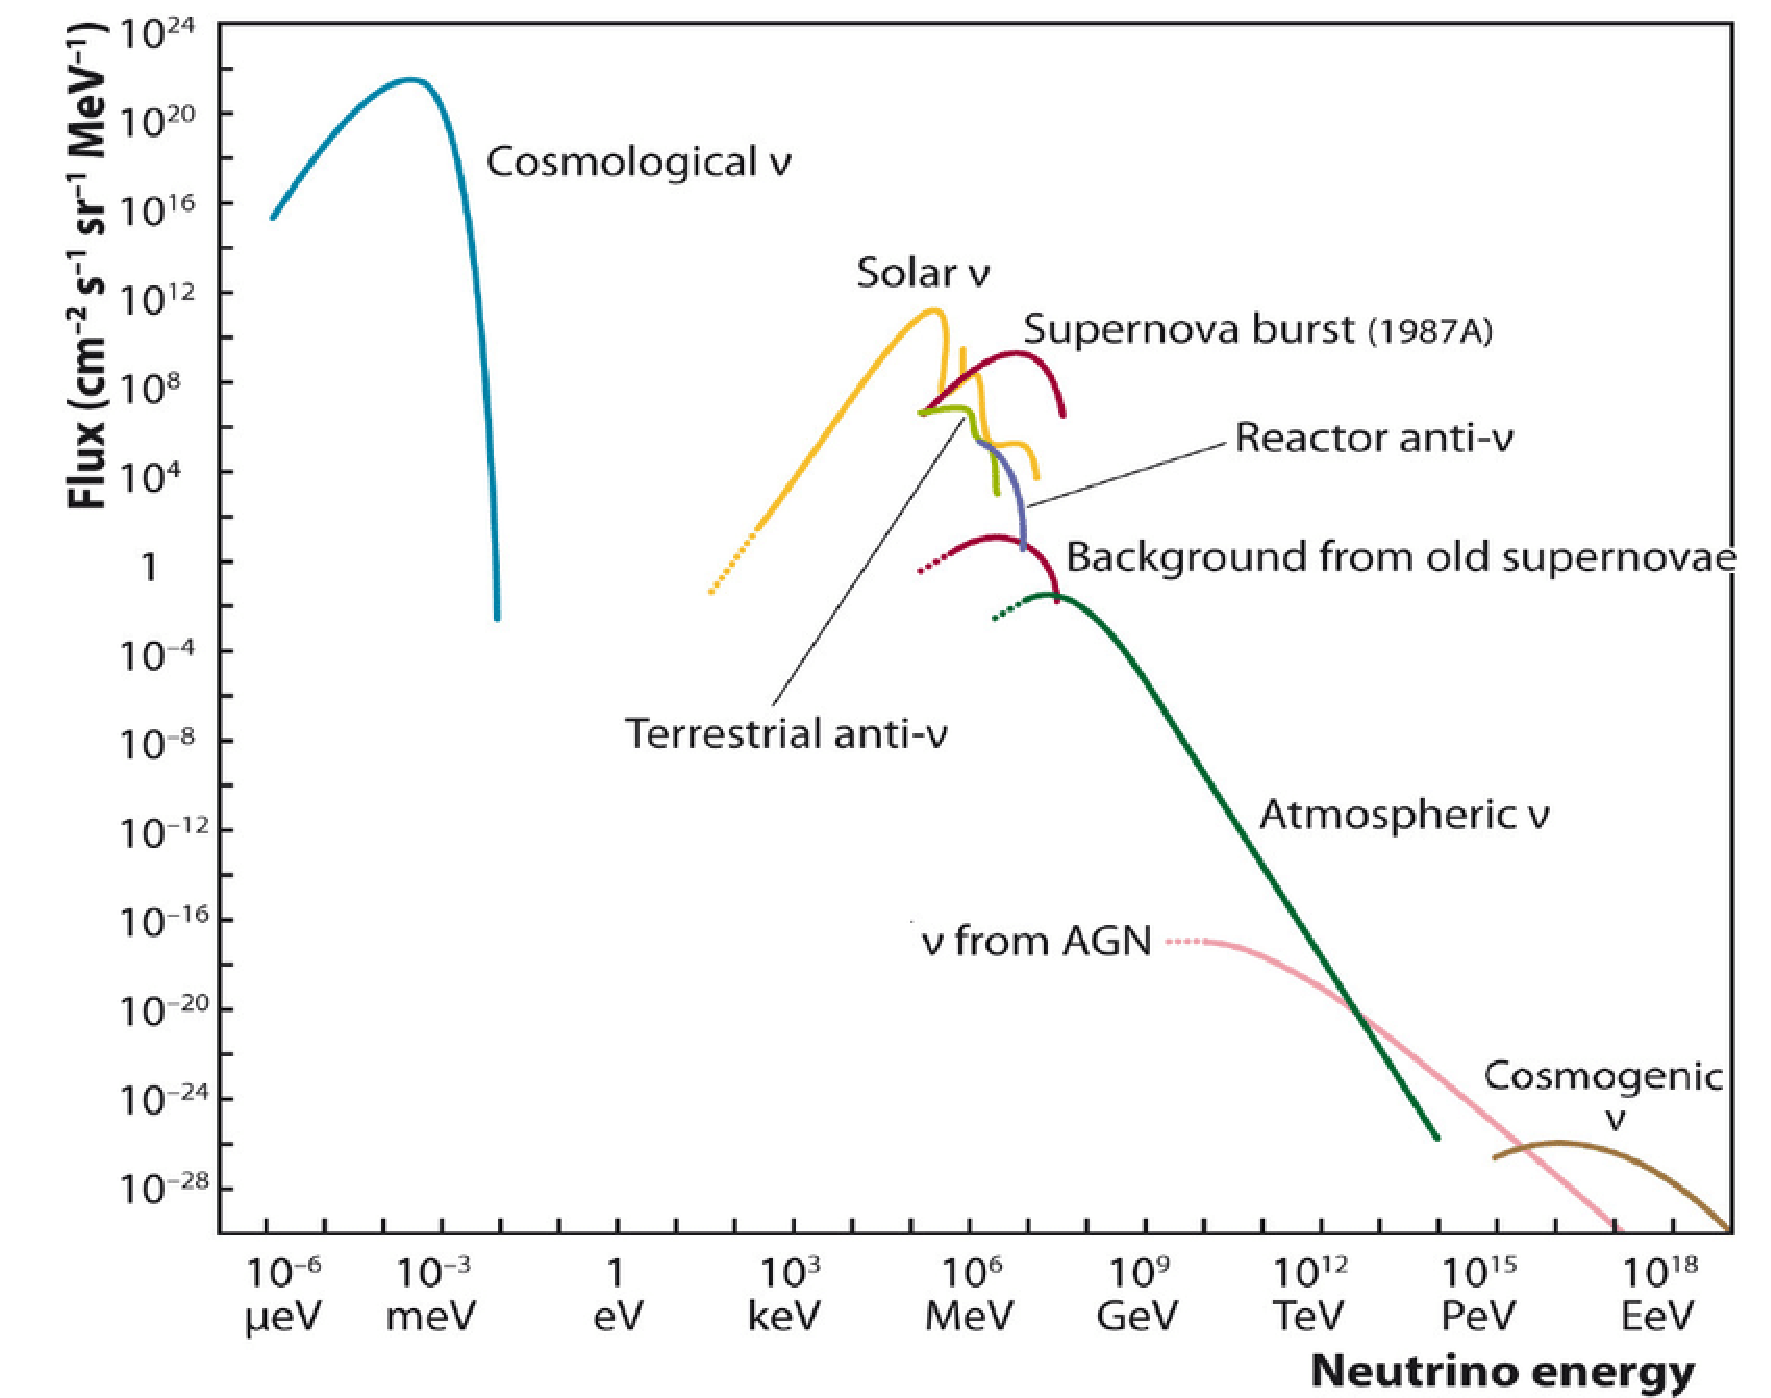
\includegraphics[height = 0.5\textwidth]{neutrinofluxes.pdf}
	\caption{Less neutrinos will be observed for higher energies \citeFig{NeutrinoFlux}}
	\label{figure:Neutrino fluxes}
\end{figure}
\subsection{Cosmological/Primordial neutrinos}
The first source of neutrinos we'll talk about is the one in blue to the left of the figure
termed the \textit{Cosmological neutrinos}: 
the neutrino version of the CMB (Cosmic Microwave Background).
To understand this source we'll have to go back all the way to just after the big bang:
The very early universe was hot and dense. As a result, interactions among particles
occurred much more frequently than they do today. As an example, a photon today
can travel across the observable universe without deflection or capture, so it has a
mean free path greater than $10^{26}$ m. When the universe was 1 second old, though, 
the mean free path of a photon was about the size of an atom. Thus in
the time it took the universe to expand by a factor of 2, a given photon interacted
many, many times. These multiple interactions kept the constituents in the universe
in thermal equilibrium. But as the universe expanded there were times when reactions could
not proceed rapidly enough to maintain equilibrium conditions, these particles then fell out
of thermal equilibrium. This falling out of equilibrium is termed \textit{decoupling}.
And we're interested in when neutrinos decoupled.
Neutrinos were kept in equilibrium through the interaction 
\begin{equation}
	\nu e \leftrightarrow \nu e
\end{equation}
Up until the universe cooled down to about 1MeV when they decoupled.
To estimate the temperature of the neutrinos who decoupled at the start of the universe, 
we can take a look at conservation of entropy \cite{Dodelson} from which we'll find that
the temperatures are related by:
\begin{equation}
	T_\nu = \left(\frac{4}{11}\right)^{1/3}T_\gamma
\end{equation}
Note that they decoupled before the photons, making them lower in temperature.
As $T_\gamma$ is the CMB temperature which, nowadays, is measured to be around
2.7K or $2.3\times10^{-4}$MeV. This would imply $T_\nu = 1.66\times 10^{-4}$MeV which
is roughly where the peak flux is located.  These primordial neutrinos are thus very
low in energy.
\subsection{Solar neutrinos}
The sun fuses elements via the pp chain reaction to release energy and thus
keeping itself from collapsing in on itself. In most of the various fusion
steps, neutrinos get released as is shown in figure
\ref{fig:SunFusion} where the neutrinos are electron
neutrinos.
\begin{figure}
	\centering
	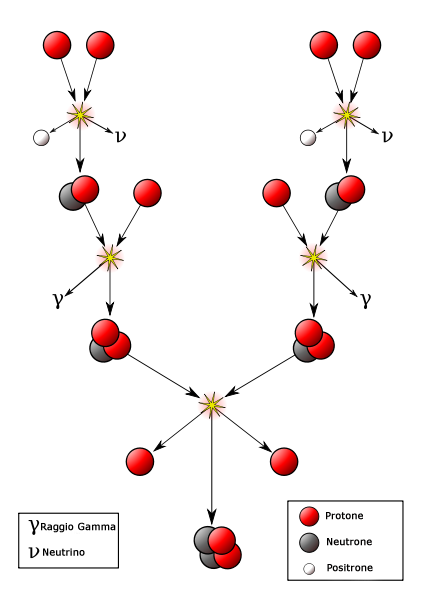
\includegraphics[width=0.4\textwidth]{figures/SunFusion.png}
	\caption{Two electron neutrinos get released over the full fusion cycle\citeFig{FusionIllu}}
	\label{fig:SunFusion}
\end{figure}
Now with this and some information about the sun like the pressure and mass,
the \textit{standard solar model} was made. This model predicted a certain
amount of electron neutrinos to be hitting the earth from the previously mentioned
thermonuclear fusion. It was however 3 times higher than the observed amount\cite{Cleveland_1998}, 
this was called the \textit{Solar neutrino problem}. 
The solar neutrino problem led to some hysteria as this could've meant
that the sun was dying and we'd see the aftermath only in a couple of years.
This phenomenon was theoretically resolved by assuming\cite{Bilenky2013} the 
different kinds of neutrinos to oscillate into each other on their way to
earth, i.e 2/3 of the original electron neutrinos had oscillated into mu and
tau neutrinos. But for them to oscillate into each other, they not
only require mass but each flavor also should have a different mass as can be seen
from an example 2D approximation to the transition probability\cite{Bellini_2014}:
\begin{equation}
	P(\nu_e\rightarrow\nu_\mu) = |\braket{\nu_\mu|\psi(L,T)}|^2 = c_\mu c_\mu^* = \sin ^2(2 \theta) \sin ^2\left(\frac{\Delta \phi_{12}}{2}\right)
\end{equation}
with
\begin{equation}
	\Delta \phi_{12} \approx \frac{m_1^2 - m_2^2}{2p}L
\end{equation}
In full generality (3D):
\begin{equation}
	\ket{\nu_\alpha} = \sum_iU_{\alpha i} \ket{\nu_i}
\end{equation}
With $U_{\alpha i}$ the Pontecorvo-Maki-Nakagawa-Sakata (PMNS) matrix\cite{1962PThPh..28..870M}.  This
phenomenon has been experimentally verified e.g through the discrepancy from
the observed and expected neutrino events coming from a nuclear reactor \cite{Eguchi_2003}.

It was later found that the oscillation of the neutrinos was further enhanced
through the Mikheyev–Smirnov–Wolfenstein effect, whereby neutrinos oscillate
more in matter of varying density (like the
sun)\cite{smirnov2019mikheyevsmirnovwolfenstein}.
\subsection{Supernovae}
\label{sec:supernovae}
Supernovae produce a lot of neutrinos, to understand when in a supernovae they get released
we'll have to go over the current theoretical understanding of how a supernova occurs. 

A star starts its life as a ball of pure hydrogen. At the core, due to the
gravitational pressure of the outside plasma, fusion of hydrogen into deuterium
and helium happens. Thus converting mass into energy. The pressure of this energy
counteracts the pressure of gravity and the star is stable.

When the hydrogen at the core runs out, no more hydrogen can be fused. For stars
with masses between $8M_\odot$ and $30M_\odot$ ($M_\odot$ being the mass of the sun)
the fusion of heavier elements starts, this can't keep going on however as at
some point the star starts to form the most stable element: iron. 

It costs energy to both make lighter elements than iron and heavier ones as can
be seen on the energy curve shown on figure \ref{fig:BindingEnergyCurve}.
\begin{figure}[!ht]
	\centering
	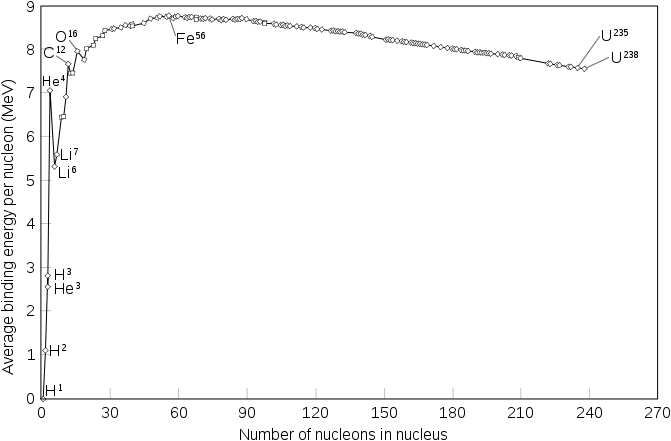
\includegraphics[width=0.5\textwidth]{Binding_energy_curve.png}
	\caption{Iron is at the top and is thus the most stable atom\citeFig{IronIllu}}
	\label{fig:BindingEnergyCurve}
\end{figure}
As the iron core builds up, the outside
pressure from the core starts to decrease as no new energy is released. This
goes on until  the threshold of an iron core with a mass of 1.4$M_\odot$ known
as the Chandrasekhar limit\cite{Chandrasekhar}\cite{weinberg1972gravitation} 
is reached and the inward pressure becomes too
large compared to the outward pressure, making the electrons surrounding the
iron core fuse with the protons (uud), creating neutrons (udd) and neutrinos,
diagrammatically shown in figure
\ref{fig:CoreFusion}.
\begin{figure}[h]
	\centering
	\begin{tikzpicture}
	\begin{feynman}
	\vertex (a0){u};
	\vertex[right=2cm of a0] (am) ;
	\vertex[right=2cm of am] (a1) {d};
	\vertex[above=2cm of am] (bm);
	\vertex[above=2cm of a0] (b0){$e^-$};
	\vertex[right=2cm of bm] (b1){$\nu_e$};
	\diagram* {
		{[edges=fermion]
			(a0) -- (am) -- (a1)
		},
		{[edges=fermion]
			(b0) -- (bm) -- (b1)
		},
		{[edges=boson,edge label=$W^+$]
			(am) -- (bm)
		}
	};
	\end{feynman}
	\end{tikzpicture}
	\caption{fusion of protons with surrounding electrons into neutrons via charged current exchange}
	\label{fig:CoreFusion}
\end{figure}\\
This last part happens in a split second as the collapse goes at 25\% the speed
of light, creating a very dense neutron star (3000km in diameter iron core to
30km in diameter neutron star) and up to $10^{52}$ ultra-relativistic
neutrinos, carrying up to 99\%\footnote{$\approx$1\% is released as kinetic energy, only 0.001\% as
electromagnetic radiation} of the released energy
\cite{Melson_2015}. As the density has suddenly increased so much,
there's a huge distance of pure vacuum between the plasma outer layer and the
(now) neutron star. This plasma starts free-falling inwards, also at 25\% the
speed of light whilst the neutrinos carrying tremendous amounts of energy start
going outward from the neutron stars core.

The neutrinos then collide with the plasma resulting in what we observe as a
"supernova", wrongly thought of by Kepler as being a "new (nova) star", rather
being a violent death of an old star.

This is quite unexpected as neutrinos rarely interact, it's only as the
incoming plasma is so dense and due to the tremendous amount of neutrinos that
collisions happen at all. Some, however, escape and will be visible on earth
in our neutrino detectors $\approx$ 18h before the light escapes the exploding
star.

Neutrino observatories can thus be useful to know where to point our various
telescopes before the supernova is actually visible in the night sky.
\subsection{Background from old supernovae}
Also termed the \textit{diffuse supernova neutrino background} (DSNB), as the
universe is quite old various supernovae have happened over it's lifetime, each generating
a lot of neutrinos as was discussed in section \ref{sec:supernovae}. 
This is postulated to have generated a continuous neutrino background\cite{Beacom_2010}.
\subsection{Atmospheric neutrinos}
\label{sec:AtmosphericNeutrinos}
Before we can talk about atmospheric neutrinos it's necessary to discuss \textit{cosmic rays}.
Cosmic rays are ionized nuclei of which 90\% are protons, 9\% are alpha particles and
the rest are heavier nuclei. Almost all of them originate from outside the solar system but
from within our galaxy. The few particles that do come from our solar system can be temporally
linked to violent events on the sun. Contrarily, the particles coming from outside
our solar system show an anti-correlation with the sun as they can more easily reach the earth
if solar activity is low.
It has been observed that the major components of the cosmic ray elements
roughly follow an inverse power law in energy, with differential flux \cite{gaisser_engel_resconi_2016}
\begin{equation}
	\frac{dN}{dE} \propto E^{-(\gamma+1)}
\end{equation}
Cosmic rays' particles hit the earth's atmosphere with a flux of about 1000 rays per
square meter per second and interact with atomic nuclei, creating showers of particles. 
Many of these showers consist of
particles which are unstable and produce neutrinos when they decay. These
neutrinos are what's called \textit{Atmospheric neutrinos}.  Most notably
neutrinos can be produced together with muons in the two-body decays of charged
pions and kaons wherever these hadronic interactions occur.  The most important
production channels and their branching ratios for neutrinos are:
\begin{align}
	\pi^\pm &\rightarrow \mu^\pm + \nu_\mu(\bar{\nu}_\mu) (\sim 100\%)\\
	K^\pm &\rightarrow \mu^\pm + \nu_\mu(\bar{\nu}_\mu) (\sim 63.5\%)
\end{align}
Neutrinos are subsequently also produced when these muons decay:
\begin{equation}
	\mu^\pm \rightarrow e^\pm + \nu_e(\bar{\nu}_e) + \bar{\nu}_\mu(\nu_\mu)
\end{equation}
which is a process mainly happening at low energies in the atmosphere.  As the
Kaons are CP violating particles, a beam of neutral kaons produced by cosmic
rays will decay in flight making the short-lived $K_S$ (K-Short) disappear and leave a
pure beam of long-lived $K_L$ (K-Long) \cite{griffiths2008introduction}.  Another decay
mode which is therefore important and the dominant source for electron neutrinos for
energies $E_\nu \geq 1$GeV is the $K_L$  decay
\begin{equation}
	K_L \rightarrow \pi^{\pm}e^\mp\nu_e(\bar{\nu}_e)
\end{equation}
The atmospheric neutrino spectrum shown in figure \ref{figure:Neutrino
fluxes} roughly follows a power spectrum as the cosmic ray flux follows a power
spectrum. But the correspondence isn't one-to-one as, due to the difference in
kinematics, the contribution from kaons to neutrinos is significantly more
important than to muons, especially at high energies \cite{gaisser_engel_resconi_2016}.

How well can we detect these atmospheric neutrinos coming from cosmic rays?
The primary way to detect neutrinos is through neutrino-nucleon interactions.
The cross section for producing a charged lepton
\cite{gaisser_engel_resconi_2016} in the 1-3000 GeV region is
\begin{equation}
	\sigma \approx 0.5\times 10^{-38} cm^2\times E_\nu (GeV)
\end{equation}
The neutrino flux at 1 GeV is $\sim$ 1cm$^{-2}$s$^{-1}$ from all directions, the interaction rate for
atmospheric neutrinos is thus of the order:
\begin{equation}
	\sim 100\frac{\nu\text{-interactions}}{\text{kT} yr}
\end{equation}
With kT denoting kilotons, therefore detectors of a kiloton or more sensitive
volume are required to study interactions of cosmic ray
neutrinos\cite{GreisenAndReines}.

\subsection{neutrinos from AGNs}
An AGN (active galactic nucleus) is deemed to be the reason why several abnormal galaxies exist with
an extra bright (and mostly variable) light source in their core which even the biggest of telescopes
can't spatially discern. The general consensus is that this phenomenon is caused by one particular
kind of object: a supermassive black hole (a black hole with a mass of at least 105M$_\odot$) surrounded with
a close torus of dust and gas\cite{Shields_1999}.
This torus of gas is called an \textit{accretion disc} and is an enormous source of energy. The conversion
of potential energy of the incoming gas to highly energetic radiation is a very complex physical process
in which we have to account for various factors like gravitational instabilities, magnetic fields, hydrodynamical
turbulence,etc. It thus produces a spectrum that's quite complex.
It would appear that the luminosity of an AGN would increase indefinitely with incoming mass, but this process is 
limited: if too much matter accretes on the black hole, the radiative pressure becomes too massive and the 
matter on the disc gets blown away. This phenomenon is termed a \textit{black hole outburst}.

The emission of high energy neutrinos from AGNs rests solely on the premise
that relativistic protons of sufficiently high energy and energy density in the
AGN's accretion disc will be present \cite{NASANeutrinos} as they may interact
to create e.g pions whom decay into neutrinos. A direct consequence of the occurrence of these
relativistic protons is the production of $\gamma$-rays of similar energies to
those of the neutrinos, thus high energy neutrino- and $\gamma$-ray astronomy are
closely related.  However, even though $\gamma$-ray photons can be produced
in the absence of relativistic protons (e.g via high energy electrons),
neutrinos can not.  Thus the detection of these high-energy neutrinos (which
might have already been detected \cite{AGNNeutrino}) will provide unique
information about the workings of AGNs.
As these ultra high energy neutrinos get produced near the source (the AGN)
they are what's called \textit{astrophysical neutrinos}

\subsection{Cosmogenic neutrinos}
In contrast to the previous source of UHE (Ultra High Energy) neutrinos which
was generated at the source, called \textit{astrophysical neutrinos}, we'll now
talk about UHE neutrinos whom are generated through the interaction of
ultra-high energy cosmic rays during propagation with the cosmic microwave or
other photon backgrounds termed \textit{cosmogenic neutrinos}.  

If a proton has sufficiently high energy, the cross
section to interact with the CMB becomes
non-negligible and it may scatter off the photons to
resonantly produce a $\Delta^+$ baryon.  This resonance has enough mass to
dominantly decay to a pion and a nucleon\cite{M_ller_2019}:
\begin{align}
	\Delta^+ &\rightarrow \pi^0 + p^+ \ \ (2/3)\\
	\Delta^+ &\rightarrow \pi^+ + n \ (1/3)
\end{align}
Of which the charged pion decays to neutrinos as previously mentioned in 
\ref{sec:AtmosphericNeutrinos}, whom are consequently very high in energy.
This phenomenon is also predicted to cause the so-called Greisen–Zatsepin–Kuzmin\cite{Zatsepin}\cite{Greisen} 
limit. As, due to this interaction, there would be a limit to the energy a cosmic ray proton might have
and still pass the intergalactic medium from another galaxy to ours. This limit is theorized to be
$5\times10^{19}$eV (50 EeV). 
